\documentclass[12pt]{scrartcl}

\usepackage{amsthm}
\usepackage{amsmath}
\usepackage{graphicx}

\title{Lecture Notes week 3}
\author{\"Omer \c Sakar}
\date{\today}

\newtheorem{defi}{Definition}
\newtheorem{theo}{Theorem}



\begin{document}
\maketitle
\tableofcontents
\newpage

\section{Lecture 1}

\subsection{Bayes' Rule}
Given events $A$ and $B$:\newline

\begin{defi}
 	The Conditional Probability $P(A | B) = \frac{P(A \cap B) }{P(B)},\ 	 with\ P(B)\ >\ 0.$
\end{defi}

\begin{figure}[h]
	\centering
	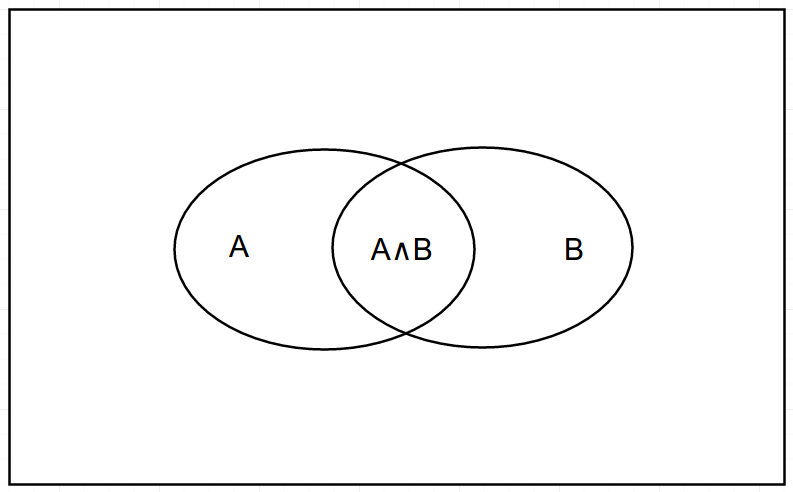
\includegraphics[width=0.3\textwidth]{./images/venn_diagram.png}
	\captionof{figure}{Visual representation of Bayes' Rule}    
\end{figure}

\noindent Example: There are 40 Math students of which 15 are girls and there are 50 Computer Science students of which 10 are girls.\newline
Let $A\ =\ randomly\ chosen\ student\ is\ a\ girl$ and $B\ =\ randomly\ chosen\ student\ is\ a\ math\ student$.
\newline

$P(A | B) = \frac{P(A \cap B)}{P(B)} = \frac{\ \ \frac{15}{90}\ \ }{\frac{40}{90}} = \frac{3}{8}$\newline

\noindent And from Bayes' Rule follows $\Rightarrow P(A \cap B) = P(A | B)\cdot P(B) = P(B|A)\cdot P(A), P(A) > 0$.

\noindent Thus we can rewrite it as:
\begin{defi}
 	The Conditional Probability $P(B | A) = \frac{P(A | B)\cdot P(B) }{P(A)}.$
\end{defi}

\subsubsection{Full Probability Formula}
\begin{defi}
	$P(A) = P(B) \cdot P(A | B) + P(\bar{B})\cdot P(A | \bar{B})$
\end{defi}
\noindent Example: $P(B | A) = \frac{P(A | B)\cdot P(B)}{P(A)} = \frac{\ \frac{40}{90}\cdot \frac{3}{8}\ }{\frac{25}{90}} = \frac{3}{8}$\newline

\subsection{A Herding Experiment}
Envelope 1 contains 8 red and 4 blue domino pieces (R) and envelope 2 contains 4 red and 8 blue domino pieces (B).\newline
$P(R) = P(B) = \frac{1}{2} $\newline
The first person that draws either a red or blue piece.\newline
$P(R | (saw) blue) = \frac{P(blue | R)\cdot P(R)}{P(blue)}$.

\noindent$P(blue) = P(R)\cdot P(blue |R) + P(B)\cdot P(blue | B) = \frac{1}{2}\cdot \frac{4}{12} + \frac{1}{2}\cdot \frac{8}{12} = \frac{1}{2}$

\noindent$P(R | blue) = \frac{\frac{4}{12}\cdot \frac{1}{2}}{\frac{1}{2}} = \frac{1}{3} < \frac{1}{2}\
 and\ P(B | blue) = \frac{\frac{8}{12}\cdot \frac{1}{2}}{\frac{1}{2}} = \frac{2}{3} > \frac{1}{2}$



\noindent Now lets look at when a second person draws.
\begin{defi}
	$D_{i} = \{blue\}\ or\ \{red\}\ -\ what\ person\ i\ says\ they\ saw$
\end{defi}
\begin{defi}
$E_{i} = \{blue\}\ or\ \{red\}\ -\ what\ person\ i\ saw$
\end{defi}
\noindent Lets say that the first person says what he sees ($D_{1} = E_{1}$)

\noindent$P(B | blue, blue) = \frac{P(B)\cdot P(blue, blue | B)}{P(blue, blue)}$

\noindent$P(blue, blue) = \frac{1}{2}\cdot (\frac{2}{3})^{2} + \frac{1}{2}\cdot (\frac{1}{3})^{2} = \frac{5}{18}$

\noindent Thus $P(B | blue, blue) = \frac{\frac{1}{2}\cdot (\frac{2}{3})^{2}}{\frac{5}{18}} = \frac{4}{5} > \frac{1}{2}$

\noindent Conclusion: If $D_{1} = \{blue\}$ and $E_{2} = \{blue\} \implies D_{2} = \{blue \}$\newline

\noindent $P(R) = P(B) = \frac{1}{2}$\\
$P(B | blue, red) = \frac{P(B)\cdot P(blue, red | B)}{P(blue, red)} = \frac{\frac{1}{2}\cdot \frac{2}{3}\cdot \frac{1}{2}}{ \frac{1}{2}\cdot \frac{2}{3}\cdot \frac{1}{2} + \frac{1}{2}\cdot \frac{2}{3}\cdot \frac{1}{2}} = \frac{1}{2}$\\
$D_{1} = \{blue\}, E_{2} = \{red\} \implies D_{2} = \{red\}$

If your opinions differ (blue, red or red, blue)then you are back at the initial situation. Thus the third person will be equivalent to the first person.\\


\noindent Let $D_{1} = D_{2} = \{blue\}$. If $E_{3} = \{blue\} \implies D_{3} = \{blue\}$ 
If $E_{3} = \{red\}$, then $P(R|blue,blue,red) = \frac{P(R)\cdot P(blue,blue,red | R)}{P(blue,blue,red)} = \frac{\frac{1}{2}\cdot \frac{1}{3}\cdot \frac{1}{3}\cdot \frac{2}{3}}{\frac{1}{2}\cdot \frac{1}{3}\cdot \frac{1}{3}\cdot \frac{2}{3} + \cdot \frac{1}{2}\cdot \frac{2}{3}\cdot \frac{2}{3}\cdot \frac{1}{3}} = \frac{2}{6} = \frac{1}{3} < \frac{1}{2}$.
Thus when $E_{3} = \{red\} \implies D_{3} = \{blue\}$.
Now the cascade has started, which also means $4th person \equiv 3rd person$.



\noindent$P(B\ cascade| R) = \frac{1}{3}\cdot \frac{1}{3} + (\frac{1}{3}\cdot \frac{2}{3})\cdot 2\cdot \frac{1}{3}\cdot \frac{1}{3} + 
(\frac{1}{3}\cdot \frac{2}{3}\cdot 2)^{2}\cdot \frac{1}{3}\cdot \frac{1}{3} + \cdots
= \frac{1}{9}\cdot \frac{1}{1 - \frac{4}{9}} = \frac{1}{5} \equiv 20\%$
\subsection{Genral Cascade Model}
Example: Adopting a product\newline
1) Let B be bad and G be good. We estimate $P(B) = 1-p$ and $P(G) = p$.\newline
2) And let $v_{g}$ be if we guess G right and $v_{b}$ if we guess B right.\newline
$v_{g}\cdot p + v_{b}\cdot (1-p) = 0$ - Expected Reward. Rewritten it looks like $v_{b} + (v_{g} - v_{b})\cdot p$.\newline
It is accepted if $P(G|signal) > p$ and rejected if $P(G | signal) < p$.

\noindent 3) low(L) and high(H)
\begin{table}[h]
\centering
\begin{tabular}{|l|l|l|}
\hline
  & B   & G   \\\hline
L & q   & 1-q \\\hline
H & 1-q & q  \\\hline
\end{tabular}
\caption{With q $> \frac{1}{2}$}
\label{my-label}
\end{table}

\noindent $P(L|B) = q > \frac{1}{2},\ P(H|B) = 1-q$. $P(L|G) = 1-q,\ P(H|G) = q > \frac{1}{2}$.\newline

\noindent First person $P(G|H) = \frac{P(H|G)\cdot P(G)}{P(H)} = \frac{p\cdot q}{p\cdot q + (1-p)\cdot (1-q)} > \frac{p\cdot q}{p\cdot q + (1-p)\cdot q} = \frac{p\cdot q}{q} = p$\newline
Thus $E_{1} = \{H\}\implies D_{1} = \{G\}$\newline

\noindent Let $a+b$ - person and $S$ - signal a times H and b times L.

\noindent $P(G|S) = \frac{P(S|G)\cdot P(G)}{P(S)} = \frac{p\cdot q^{a}\cdot (1-q)^{b}}{p\cdot q^{a}\cdot (1-q)^{b} + (1-p)\cdot (1-q)^{a}\cdot q^{b}} > \frac{p\cdot q^{a}\cdot (1-q)^{b}}{p\cdot q^{a}\cdot (1-q)^{b} + (1-p)\cdot q^{a}\cdot (1-q)^{b}} = p$

\noindent This is when $a < b \iff (1-q)^{a}\cdot q^{b} > q^{a}\cdot (1-q)^{b}$ (because $q>1-q$). 

\noindent Thus when $a < b, D = \{B\}$

\noindent If $a > b \iff (1-q)^{a}\cdot q^{b} < q^{a}\cdot (1-q)^{b}$ . This would result in $P(G|S) > p \implies D = \{G\}$

\begin{figure}[h]
	\centering
	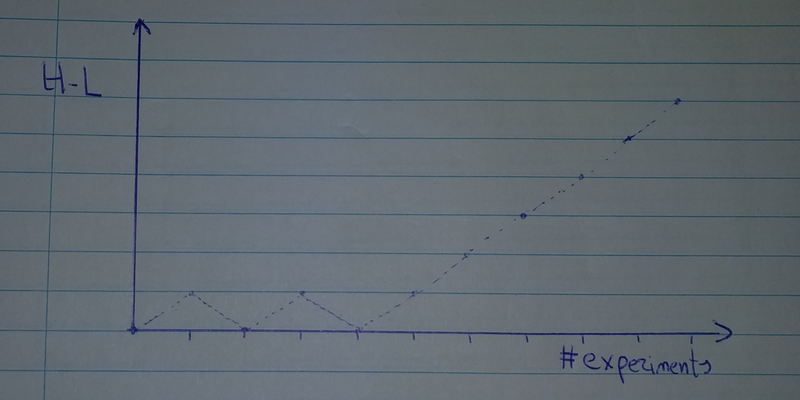
\includegraphics[width=\textwidth]{./images/graph_lecture_1.png}
	\captionof{figure}{Graph showing cascade with up = H and down = L}    
\end{figure}

\newpage
\section{Lecture 2 Network Effects} 
\begin{defi}
	Externality: welfare affected by actions of others without a "contract" (mutual agreement).
\end{defi}

\begin{defi}
	Interest: reservation price (how much you are willing to pay).\end{defi}

\begin{defi}
	Consumers: numbers between 0 and 1.
\end{defi}

When $x < y$, x has a \underline{higher} reservation price than y.
\begin{defi}
	r(x): reservation price where $0 < x < 1$.
\end{defi}

\begin{figure}[h]
	\centering
	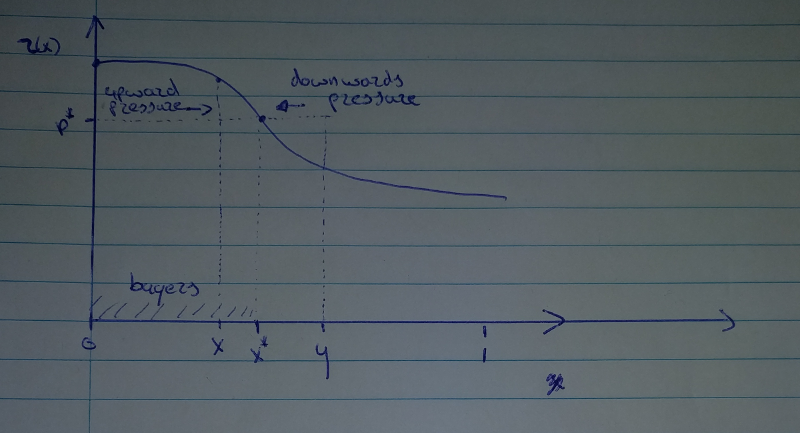
\includegraphics[width=1\textwidth]{./images/graph_res_price.png}
	\captionof{figure}{Reservation price}    
\end{figure}

\begin{defi}
	p: market price. $p \geq r(0)$ means nobody buys it and $p \leq r(1)$ means everybody buys it.
\end{defi}

\begin{defi}
	$p^{*}$: equilibrium market price. $x^{*}$ is chosen such that $r(x^{*}) = p^{*}$ - equilibrium quality.
\end{defi}

\noindent $x < x^{*} \implies r(x) > p^{*} \implies$ x wants to buy.\\
$y > x^{*} \implies r(y) < p^{*} \implies$ y regrets it (downwards implies regret).\\

\begin{defi}
	z: fraction of the population that uses the product
\end{defi}
\begin{defi}
	r(x): reservation price of x $\in [0,1]$
\end{defi}
\noindent The price  x wants to pay $p^{*} = r(x)\cdot f(z)$ (the "new" reservation price). $f(z)$ is increasing in z.\\
$f(0) = 0$ (if nobody uses the product) $\implies p(0) = r(0)\cdot f(0) = 0$

\begin{figure}[h]
	\centering
	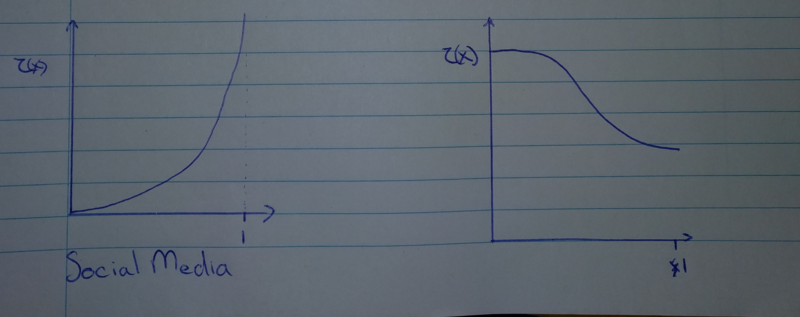
\includegraphics[width=1\textwidth]{./images/graph_social_media.png}
	\captionof{figure}{Example for social media}    
\end{figure}

So the customer expects fraction $z$ and buys the product if $r(x)\cdot f(z) \geq p^{*}$ where $p^{*}$ is the market price.\\

\subsection{Self-fulfilling expectation}
If all customers agree that fraction $f$ will buy the product and behave based on that, then the fraction of people who buys the product will be $z$.\\
How it works:\\
$z = 0: f(0) = 0 \implies \forall x\ holds\ r(x)\cdot f(0) = 0 \implies z = 0$\\ 
$x' > 0$ buys the product ($z > 0$). 
$r(x')\cdot f(z) > p^{*}$, $r(x)$ is decreasing fraction.\\
$x < x' \implies r(x) > r(x') \implies r(x)\cdot f(z) > r(x')\cdot f(z) > p^{*} \implies$ x buys.\\

\noindent Customer z has lowest intrinsic value $r(z)$ on $[0,z]$.

\noindent If $p^{*} = f(z)\cdot r(z) \implies$ self-fulfilling expectation.

\begin{figure}[h]
	\centering
	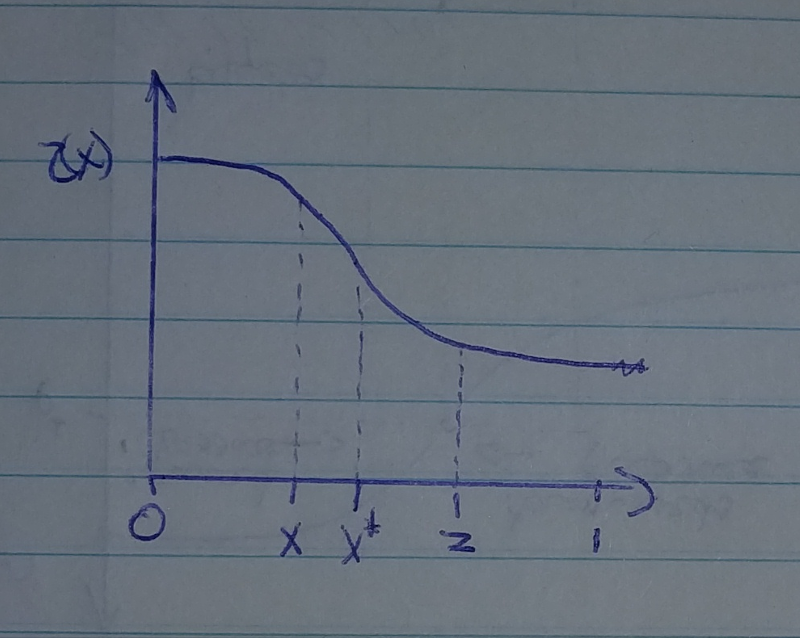
\includegraphics[width=0.4\textwidth]{./images/graph_self_fulfilling.png}
	\captionof{figure}{Reservation Price}    
\end{figure}


\noindent Suppose $p^{*} = f(z)\cdot r(x)$ for some x $\implies$ fraction x will but $\implies$ actual value for x is $f(x)\cdot r(x)$. $x < y \implies f(x)\cdot r(x) < p^{*} \implies$ x paid too much!

\noindent If $p^{*} = r(z)\cdot f(z)\ (\exists z$ (there is alwats such a $z)) \implies$ z buys $\implies x< z$ also buys $\implies$ fraction z will have it.\\

\noindent z is the fraction of the population that uses the product. $r(x)$ is the intrinsic price of $x \in [0,1]$. The price x wants to pay $p(x) = r(x)\cdot f(z) $, in other words the reservation price. $p^{*} = r(z)\cdot f(z)$ is the equilibrium.
$f(0) = 0 \implies p^{*} = r(0)\cdot f(0) = 0$, in other words equilibrium.




\noindent Example: $r(x) = 1 - x^{2},\ f(z) = z^{2}$\\
$p^{*} = r(z) = (1-z^{2})\cdot z^{2}$

\noindent $p^{*} > \frac{3}{16} \implies$ no solution\\
$p^{*} < \frac{3}{16} \implies r(z)\cdot f(z)$ has 2 solutions.

\begin{figure}[h]
	\centering
	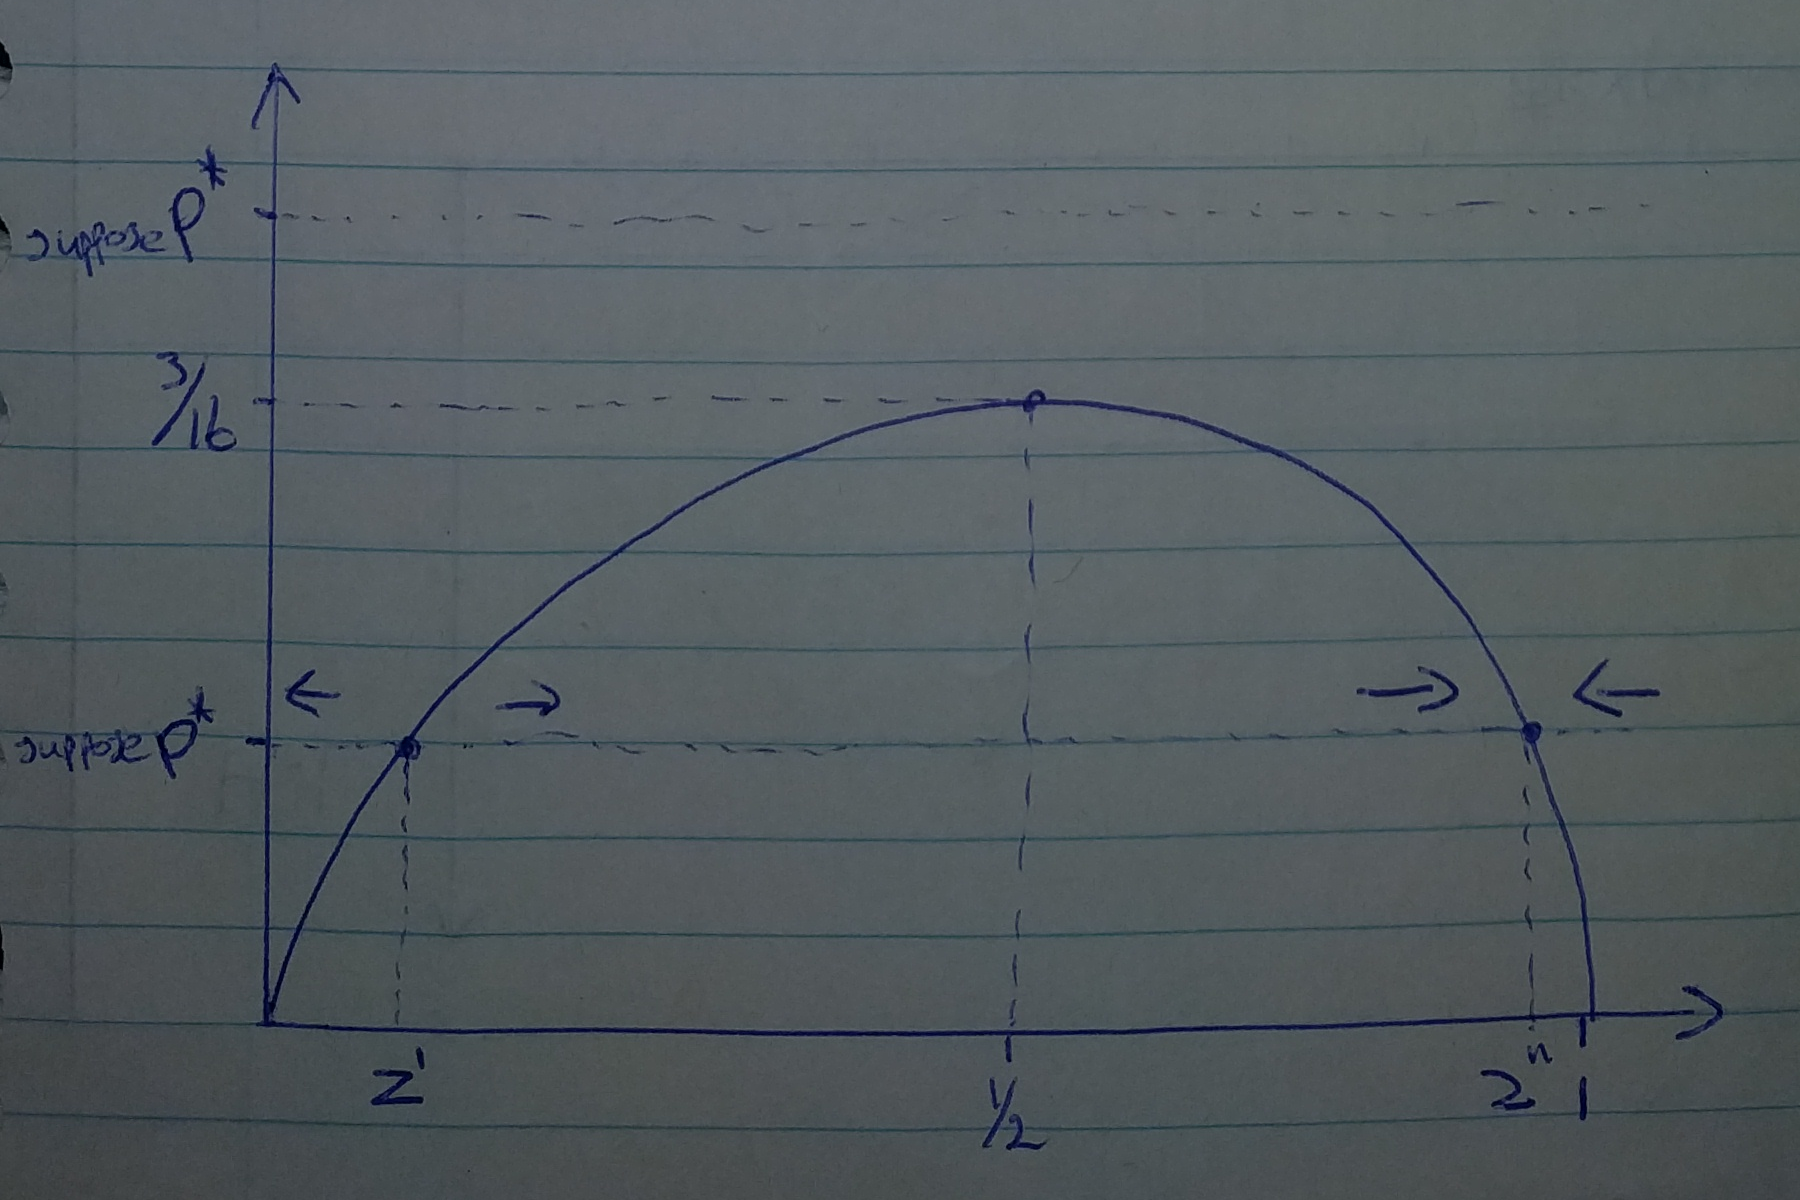
\includegraphics[width=0.9\textwidth]{./images/graph_tipping_point.png}
	\captionof{figure}{$p^{*}$}    
\end{figure}

\begin{figure}[h]
  \centering
  \begin{minipage}[h]{0.49\textwidth}
    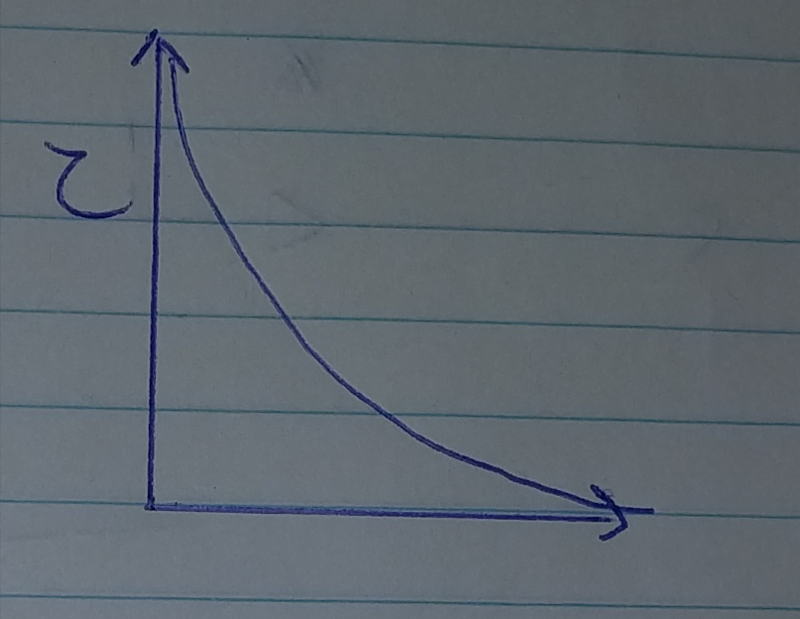
\includegraphics[width=\textwidth]{./images/graph_r.png}
  \end{minipage}
  \hfill
  \begin{minipage}[h]{0.49\textwidth}
    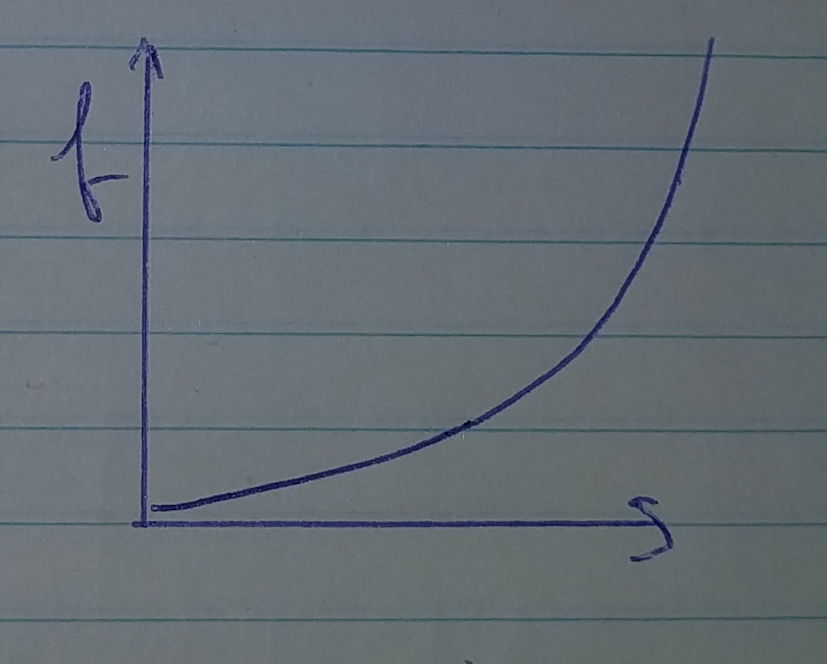
\includegraphics[width=\textwidth]{./images/graph_f.png}
  \end{minipage}
\end{figure}

\noindent We will look at different cases:
\begin{enumerate}
\item $z = 0$: This is a stable equilibrium.
\item $ 0 < z < z'$: $r(z)\cdot f(z) < p^{*} \implies$ if they have bought it, they regret it (downward pressure).
\item $z'< z < z''$: $r(z)\cdot f(z) > p^{*} \implies$ more people want the product (upward pressure).
\item $z > z''$: $r(z)\cdot f(z) < p^{*} \implies$ downwards pressure. 
\end{enumerate}

\noindent Conclusion: 0 and $z''$ are stable equilibrium and $z'$ is a tipping point.



\subsection{A Dynamic View}
x wants to purchase, thus $r(x)\cdot f(z) \geq p^{*}$. We define $\hat{z}$ as a solution for $r(\hat{z})\cdot f(z) = p^{*}$. This can be rewritten as $r(\hat{z}) = \frac{p^{*}}{f(z)}$. It holds that when $r(0) \geq \frac{p^{*}}{f(z)} \iff$ solution exists. We can also rewrite the formula to $\hat{z} = r^{-1}(\frac{p^{*}}{f(z)}) = g(z)$, ($\hat{z}$ is the fraction of people that will buy given $z$ and $p$).\\

\noindent Example: $r(x) = 1 - x^{2}, f(z) = z^{2}, \hat{z} = \sqrt{1-\frac{p^{*}}{z^{2}}}$.\\
If $z > \sqrt{p^{*}} \implies \hat{z}$ is defined and if $z \leq \sqrt{p^{*}} \implies \hat{z} = 0$. 

\noindent $q = r(x) = 1 - x^{2} \implies x^{2} = 1 - q$\\
$x = \sqrt{1-y} = r^{-1}(y)$
Remember that in these cases we have always assumed that $f(0) = 0$.

\begin{figure}[h]
	\centering
	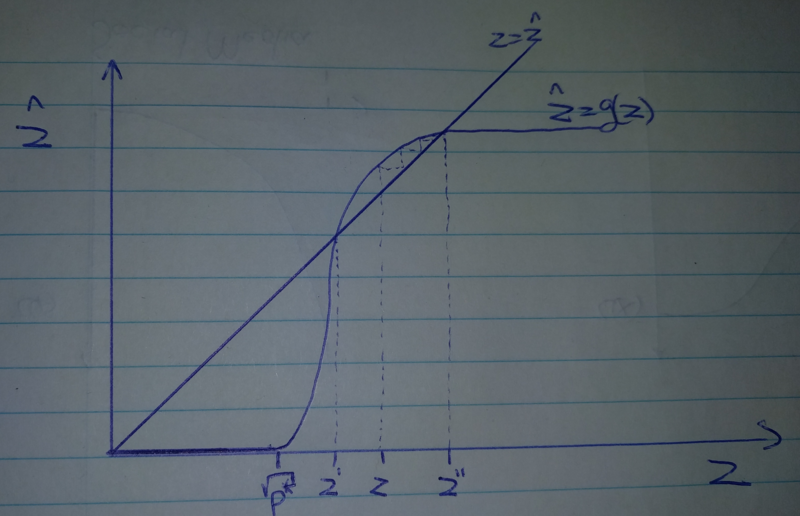
\includegraphics[width=\textwidth]{./images/graph_z_hat.png}
	\captionof{figure}{$\hat{z}$ plotted against $z$}    
\end{figure}

\end{document}




